\chapter{Intermediate Algebra}

\section{Review and Expanding on Various Topics}

Phương trình một biến bậc nhất $ax+b=c$ có thể có: một nghiệm, vô nghiệm hoặc vô số nghiệm.

\vspace{.5cm}

\hl{Graphing Linear Inequalities}: Trong hình dưới, tất cả điểm được tô màu including the line đều thỏa mãn bất phương trình.

\begin{figure}[htb!]
  \centering
  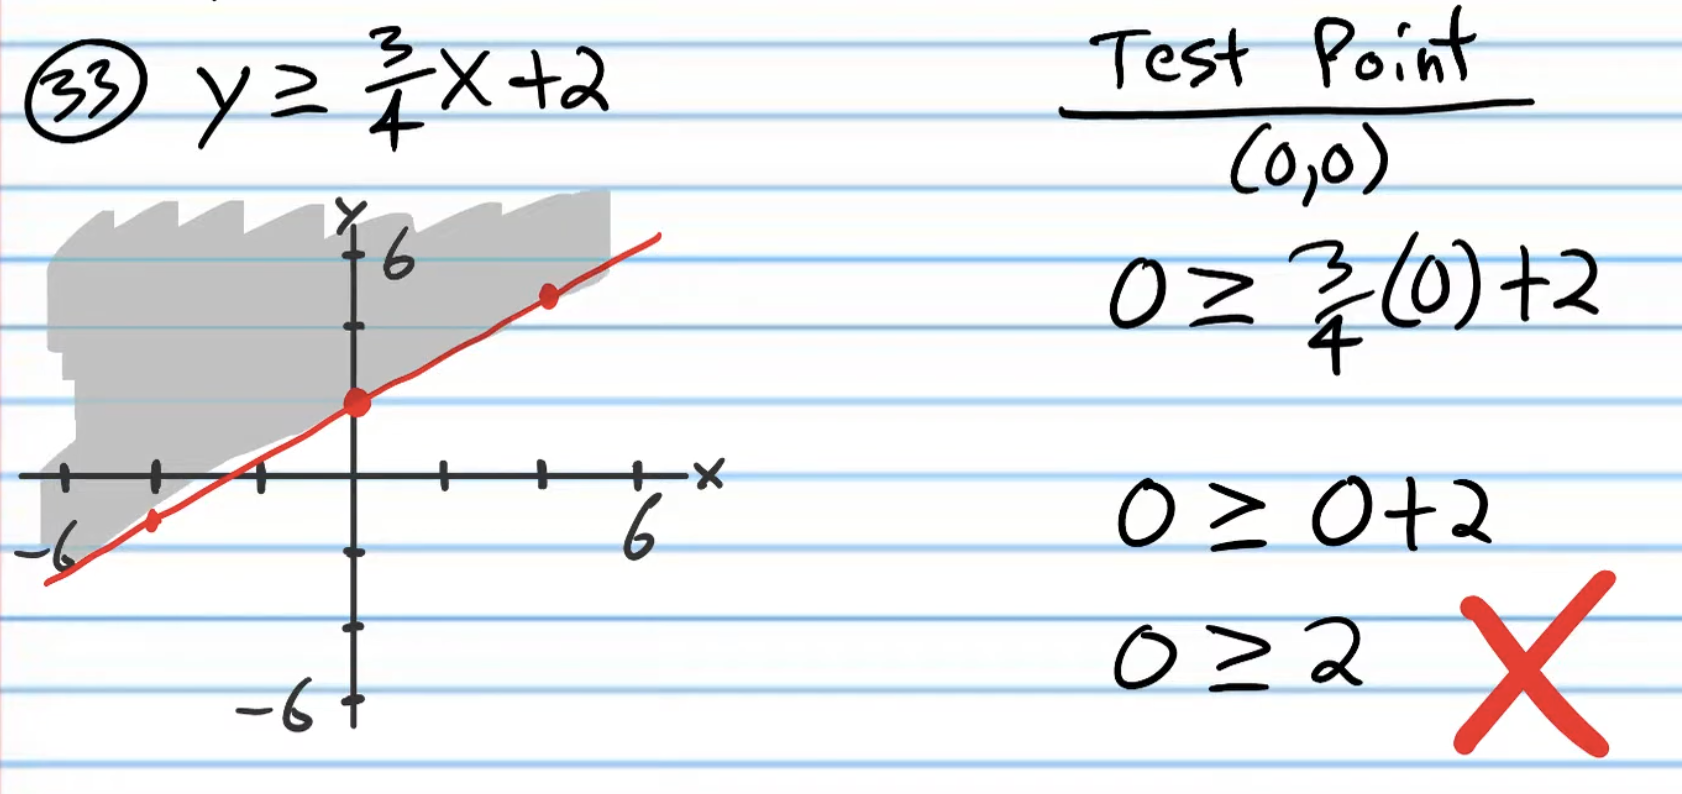
\includegraphics[width=.7\textwidth]{int0203.png}
  \caption{Graphing Inequalities}
\end{figure}

Draw the line giống như một linear equation, sau đó lấy tọa độ một điểm plug vào inequality để test coi phải tô màu phần nào. Thường chọn (0,0) cho dễ test. Nếu dựa vào greater thì tô màu phần trên, less than tô phần dưới là sai. Phải chọn test point.

\vspace{.5cm}

Draw (graph) \textbf{one variable inequality} like $2x-3>5$ thì sao? Linear Inequalities có x, y là 2D còn one variable x là 1D tức là một đường thẳng (the Number Line). Chấm một điểm rồi tô màu phần bên trái hay bên phải điểm đó thôi.

\vspace{0.6 cm}

\centerline{\textbf{\Large Graphing Systems of Linear Inequalities}}

\vspace{0.3 cm}

Two line intersect so four sections, only tô màu one section. Chọn test point phải chọn 3 điểm nằm trong 4 sections. Test point phải thỏa cả 2 bất phương trình.

Có equal thì sẽ full line, không thì vẽ dotted line.

\begin{figure}[htb!]
  \centering
  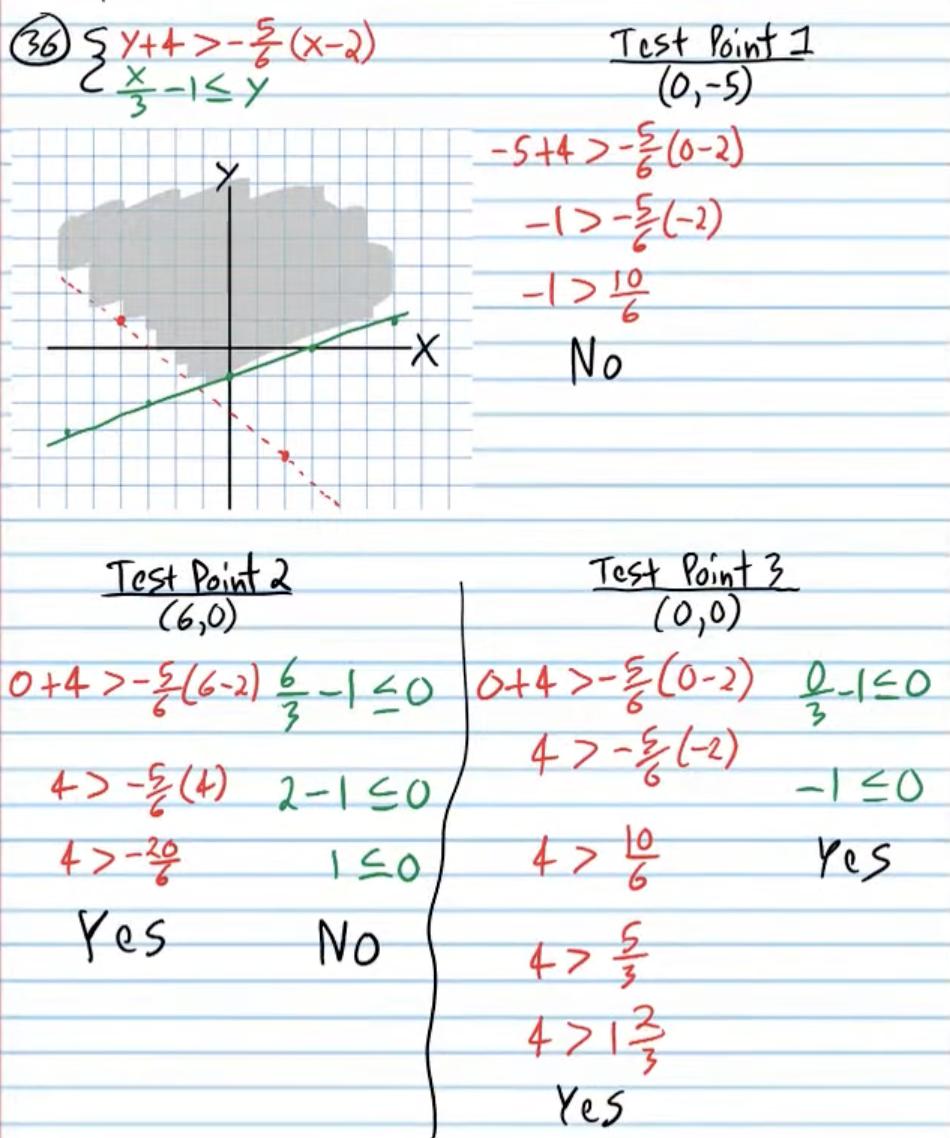
\includegraphics[width=.8\textwidth]{int0204.png}
  \caption{Graphing Systems of Linear Inequalities}
\end{figure}

\section{Solving Systems of Three Equations}

Hệ pt 3 biến cũng có tối đa một nghiệm (x, y, z), no solution, infinite solutions.

Tìm cách chuyển về hệ pt 2 biến x, y rồi giải.

Dùng substitution or elimination khử một ở 2 phương trình đầu biến nó thành hệ pt 2 biến x, y. Giải tìm x, y rồi sau đó tìm z.

\vspace{.4cm}

Bài ở dưới, khi lấy pt (a) cộng pt (c) ra $0=0$ là kết luận ngay \textbf{infinite solution}. Nhưng nếu tiếp tục làm ta sẽ phát hiện $x=1$ là constant và $y=z$ vô số nghiệm có dạng $(1, a, a)$.

\begin{figure}[htb!]
  \centering
  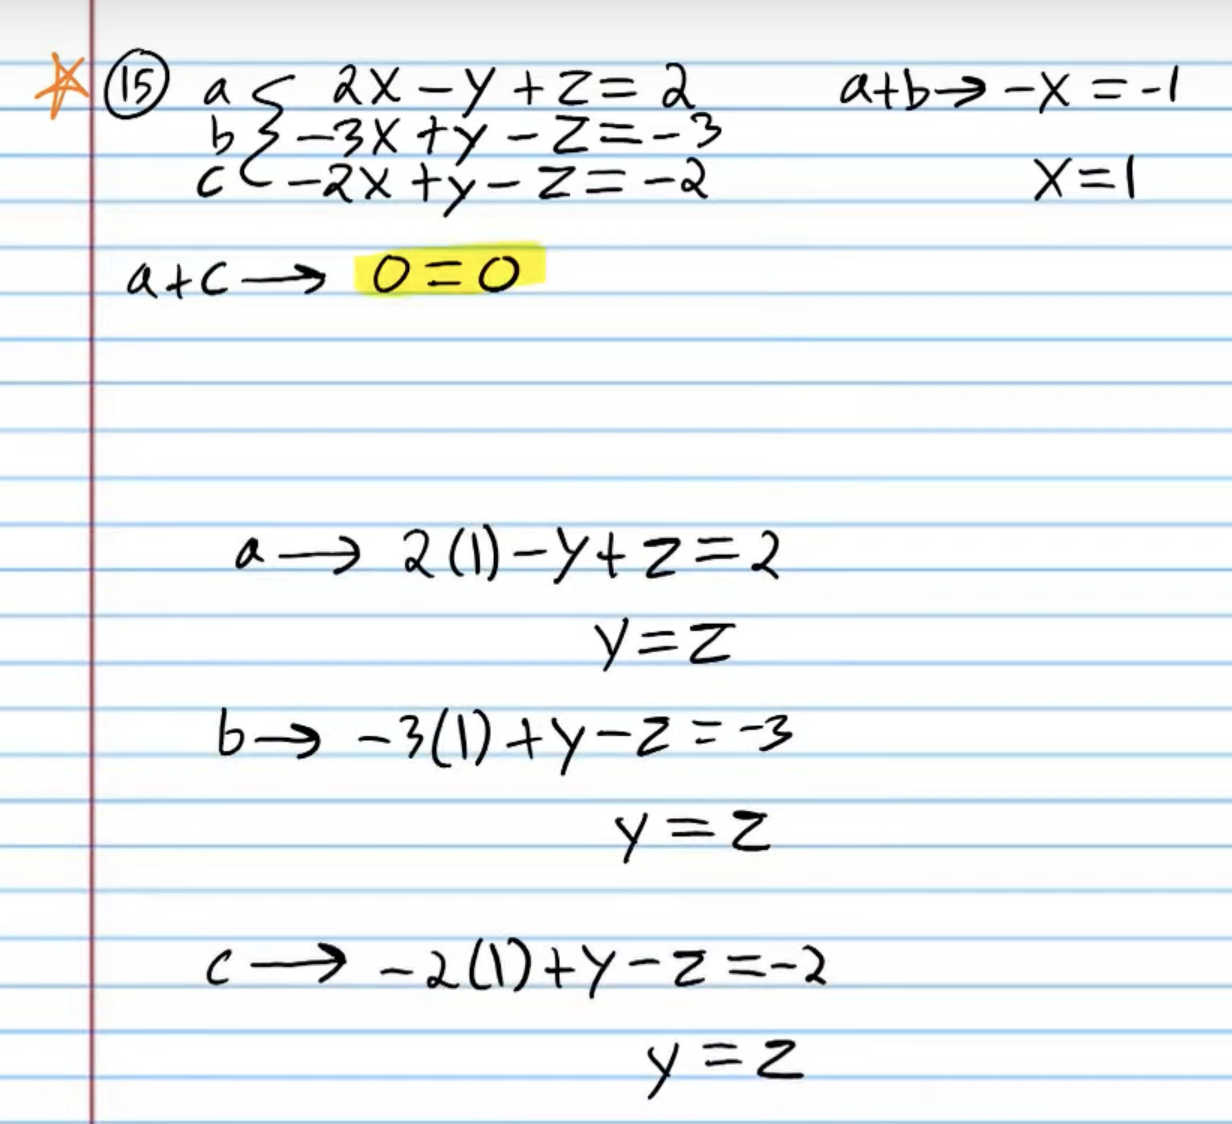
\includegraphics[width=.6\textwidth]{int0301.png}
  \caption{Bài tập}
\end{figure}

\section{Absolute Value Equations and Inequalities}

\begin{equation*}
\begin{split}
  &|x| = 8 \\
  =>\ x=8 &\text{ or } x=-8
\end{split}
\end{equation*}

\begin{align*} 
|y|+2=-3\\
|y| = -5\\
  =>\text{ No Solution.}
\end{align*}
